% !TeX root = COSTERMANS_Arnaud_Rapport_de_Stage_V.tex


\documentclass[a4paper,12pt]{article}
\usepackage[french]{babel} %translates document elements to french
\usepackage{Arnaud_C_rds}

\hypersetup{pdftitle={L3 Internship report},
pdfauthor={Arnaud COSTERMANS},
pdfcreationdate=D:20240430133559+01’00’,
pdfsubject={Internship report},
pdfkeywords={Internship, L3, SOMAIR, CanOP, Uranium extraction, Orano Mining},
}


%TODO: Description NAI
%  figure tention SIPM
% index



\setlength{\parskip}{0.5 em} %adjust the space between paragraphes to be a bit wider





% Page de garde
\begin{document}
%on repartie le document en plusieure fichier Tex pour faciliter le lecture
\begin{titlepage}
    \centering
    
    % Logo de l'Institut
    
\includegraphics[width=0.3\textwidth]{img/logo/logo_institut.jpeg} 
\includegraphics[width=0.3\textwidth]{img/logo/UPSaclay.jpg}

    % Titre du sujet
    \vspace{1.5cm}
    {\LARGE\textbf{Rapport de stage}\par}
    
    % Informations sur l'étudiant
    \vspace{1.5cm}
    {\large\textbf{Arnaud COSTERMANS}\par}
    
    % Année universitaire
    \vspace{0.5cm}
    Année universitaire : 2023-2024
    
    % Année d'études et nom de l'Institut
    \vspace{0.5cm}
    Année d'études : Promotion 2024 (L3) \\
    Licence de Science et Technologie \\
    Institut Villebon - \textit{Georges Charpak}
    
    % Informations sur le laboratoire/entreprise
    \vspace{2cm}
    
\includegraphics[width=0.2\textwidth]{img/logo/logo-orano.png}
    
    % Nom et adresse du laboratoire/entreprise
    \vspace{0.5cm}
    \textbf{Orano Mining}\\
    125 Av. de Paris, 92320 Châtillon\\
    % Nom du maître de stage
    \vspace{0.5cm}
    Maître de stage : Youcef BENSEDIK
    
    % Nom de l'enseignant référent
    \vspace{0.5cm}
    Enseignant référent : Cyril DAUPHIN
    
    % Durée du stage ou date de soutenance
    \vspace{0.5cm}
    Stage effectué du 22/04 au 13/06 (7 semaines)
\end{titlepage}
\clearpage

%\maketitle

\begin{center}

    \subsubsection*{Remerciement}
\addcontentsline{toc}{section}{Remerciement}
J'aimerais remercier Youcef BENSEDIK, qui bien que souvant occuper a toujour trouver le temps pour faire un point et m'expliquer quelque chose. J'aimerai egalement remercier Arnaud WUILBEAUX ainsi qu’Orano  de m'avoir accueilli pendant ce stage et tout les equipe qui m'on expliquer le fonctionement de certain chose, a la fois de la procedure a des methode de production.
\end{center}


\begin{abstract}
    \lipsum[1]
\end{abstract}
    

\begin{adjustwidth}{30pt}{30pt}
\end{adjustwidth}

% \vspace{50pt}
%remerciement 
\tableofcontents
% \newpage
\listoffigures
%\listoftables
\clearpage
\section{Introduction}
\lipsum[]



\section{Somaïr}
Dans cette partie, nous allons tout particulièrement nous intéresser au fonctionnement de Somaïr, la mine à ciel ouvert d'Orano au Niger, car c'est la qu'est déployé le projet CanOp et qui me faut comprendre leur procédure pour donner des suggestions cohérentes.
\subsection{L'exploration}
Avant le début de l'extraction, des géologues ont réalisé des études pour trouver d'éventuel gisement. S'ils soupçonnent la présence d'uranium, les géologues vont réaliser des campagnes de sondage successives\footnote{Soit une carotte ou un forage dans lequel on abaisser un 
sonde gamma. Cela permet d'etablire le gisment en 3D}. La maille de sondage sera à affiner jusqu'à avoir des forages espacés de 25~m. 
\subsection{L'extraction}
\label{ssec_extraction}
Si la décision de passer en production est prise alors on va venir enlever toute la roche au-dessus du gisement (50 a 70~m à Somaïr) et l’on va affiner le sondage jusqu'à une maille de 5~m*5~m qui va permettre de modéliser au mieux la distribution d'uranium dans le sol. Enfin, la fosse sera divisée en carrés de 2,5~m de large sur 2,5~m de longueur sur 0,5~m de profondeur que l'on appellera "slab" par la suite. Pour extraire ces slabs, on enterre juste assez d'explosif pour fragiliser la roche et permettre qu'une pelle mécanique puisse extraire la slab pour la charge dans un camion.
\subsection{Classification des slabs}
\begin{figure}
    
    \begin{subfigure}[t]{0.4\textwidth}
        \centering
        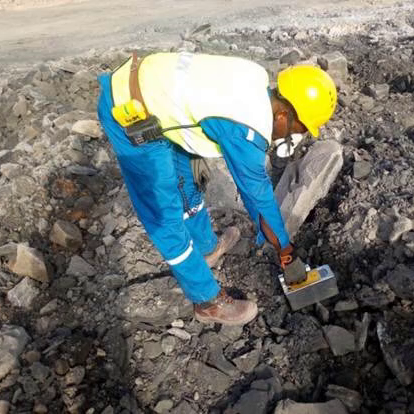
\includegraphics[height=0.3\paperwidth]{img/photo/Travail_geiger.png}
        \caption{Photo d'un operateur utilisant un compteur Geiger Müller pour mesurer la teneur en uranium d'un slab}
        \label{fig_AP_geiger}
    \end{subfigure}
    \begin{subfigure}[t]{0.6\textwidth}
        \centering
        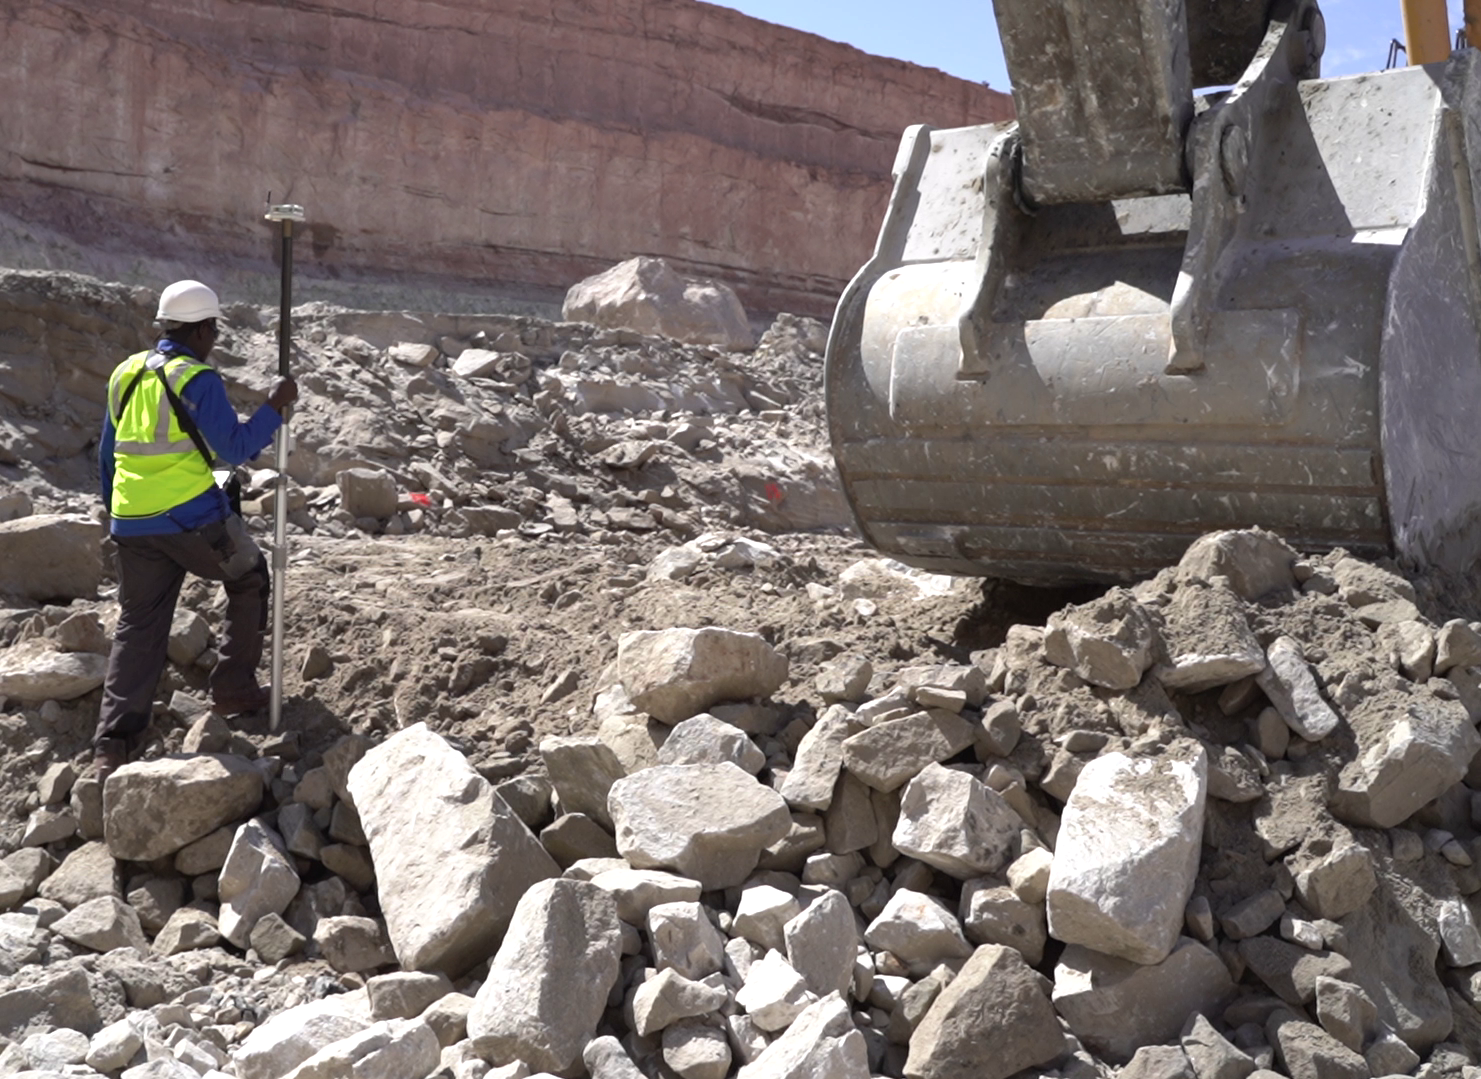
\includegraphics[height=0.3\paperwidth]{img/photo/CanOp_utilisation.png}
        \caption{Photo d'un operateur utilisant la CanOp pour mesurer la teneur en uranium d'un slab. Il porte une tablette pour voir les mesure et sa position en temps reel}
        \label{fig_AP_CanOp}
    \end{subfigure}
    \caption{Photo d'AP utilisant un compteur Geiger Müller et la CanOp}
\end{figure}
Pour savoir comment traiter ces slabs  après extraction, nous les catégorisons en 7~classes de M0 à  en fonction de leur teneur en uranium. Au début, ces teneurs étaient mesurées  Les slabs~M0 sont dites stériles, car elle contient tellement peu d'uranium que l'on ne souhaite pas les traiter. Les classes~M1 et M2 subissent un traitement que l'on dit statique, car c'est slab sont empiler et l’on attend que l'uranium descend par gravité jusqu'un bas. Enfin les slabs de classe supérieure reçoivent un traitement dynamique où en fonction de leur classe elles seront dissoutes avec plus ou moins d'acide selon leurs classes. Il est donc important de bien classer les slabs, car sinon, soit on gaspille  de l'acide ou alors il reste des l'uranium non extrait dans notre refus.
%TODO:mistakes
Avant, pour classer une slab, un Aide Prospecteur (AP) utiliser un compteur Geiger Müller en se penchant pour obtenir des mesures a plusieurs points sur le slab. Il était donc pénible de se pencher en permanence et donc en 2018 a été lancer le projet CanOp pour réduire la pénibilité de la tache.

\section{CanOp}
\label{sec_CanOp}
CanOp est le nom qui a été donné au projet de crée une sonde nouvelle génération pour la mine Somaïr au Niger. Cette sonde est composée de 3~pièces. 
\begin{itemize}
    \item 2 Sondes de rayonnement Gamma fournissent par la société Geovista
    \item une partie électronique qui inclue une batterie.
    \item Un GPS différentiel fourni par Ophelia 
\end{itemize}
Un opérateur utilise cette sonde en connexion avec une tablette pour déterminer ou extraire du minerai. 
\subsection{Les sondes Gamma}
\label{ssec_sonde}
Les sondes gamma de cet appareil proviennent de chez Ophelia et sont composées de deux parties.
\begin{figure}
    
    \begin{subfigure}{0.9\textwidth}
        \centering
        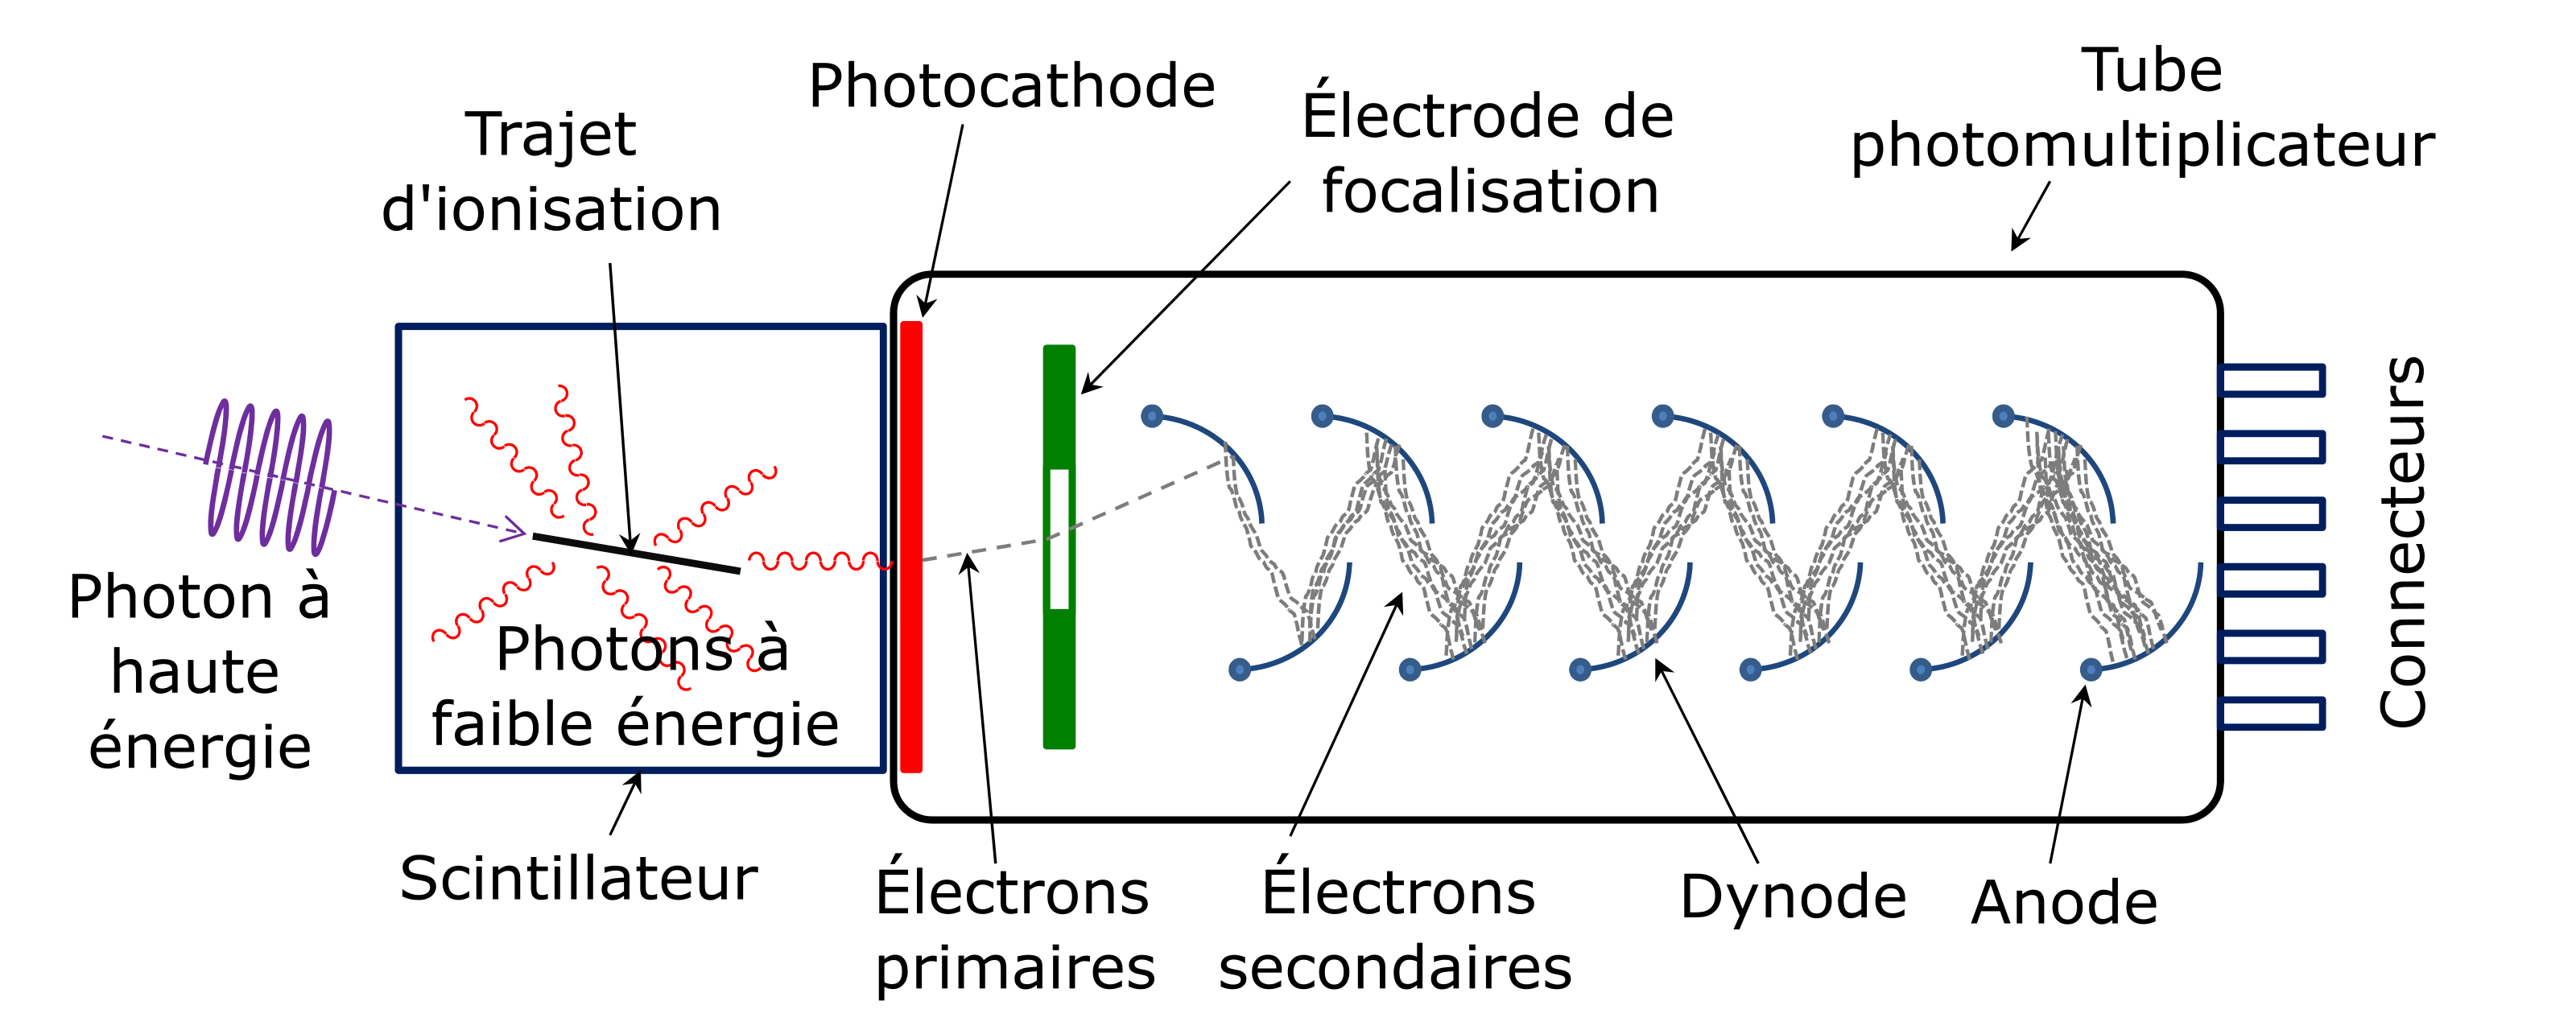
\includegraphics[width=0.9\textwidth]{img/she/Photomultiplier_coupled_to_a_scintillator_-_fr.png}
        \caption[Shema d'une sonde gamma NaI]{Schéma d'une sonde gamma NaI. Source~: \href{https://commons.wikimedia.org/wiki/File:Photomultiplier_coupled_to_a_scintillator_-_fr.png}{Qwerty123uiop}, \href{https://creativecommons.org/licenses/by-sa/3.0}{CC BY-SA~3.0}, via Wikimedia Commons}
        \label{fig_detecteur_gamma}
    \end{subfigure}
    \begin{subfigure}{0.45\textwidth}
        \centering
        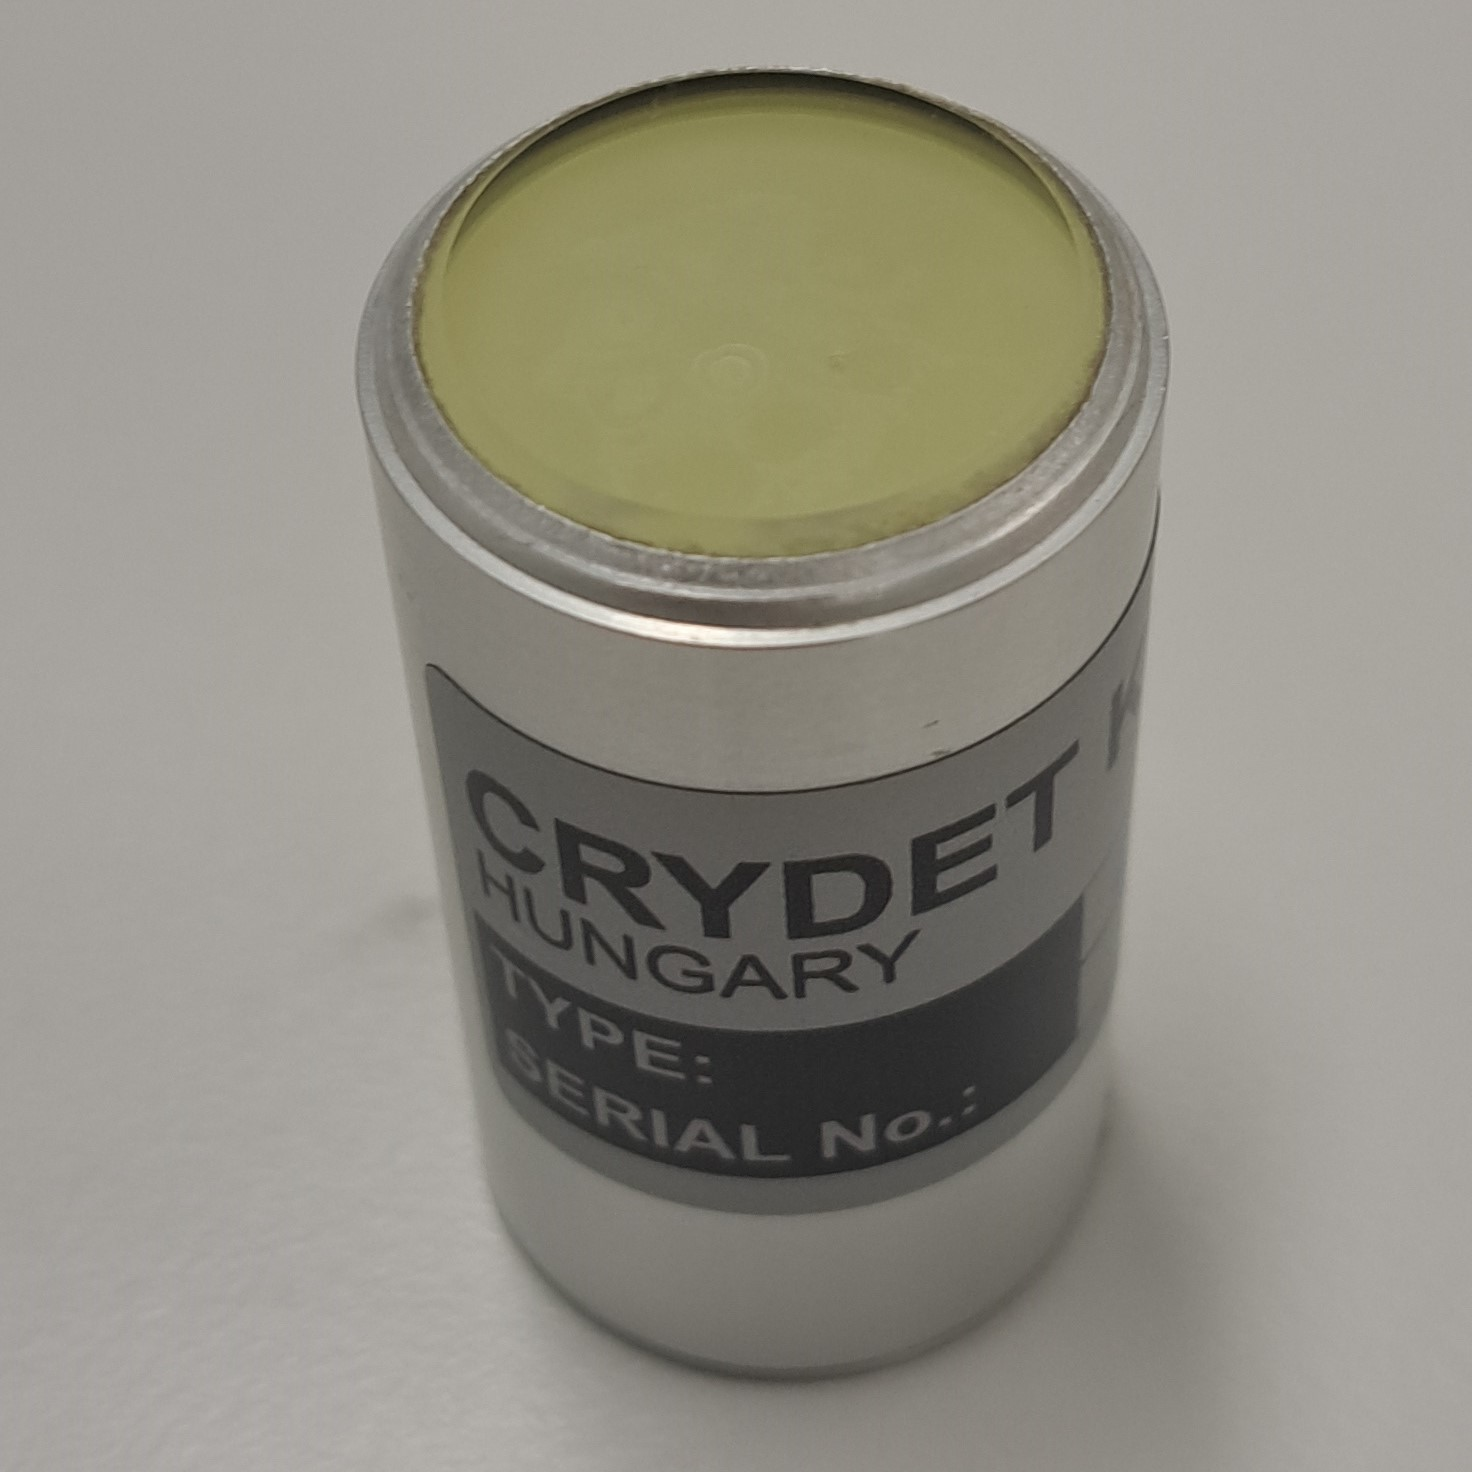
\includegraphics[trim=1cm 2cm 3cm 4cm, clip=true, totalheight=0.5\textheight, angle=90]{img/photo/Crystal.jpg}
        \caption[Photo d'un cristal NaI]{Photo d'un cristal NaI doper au thallium. Dimension~: diamètre 28*50~mm}
        \label{fig_Nai}
    \end{subfigure}
    \begin{subfigure}{0.45\textwidth}
        \centering
        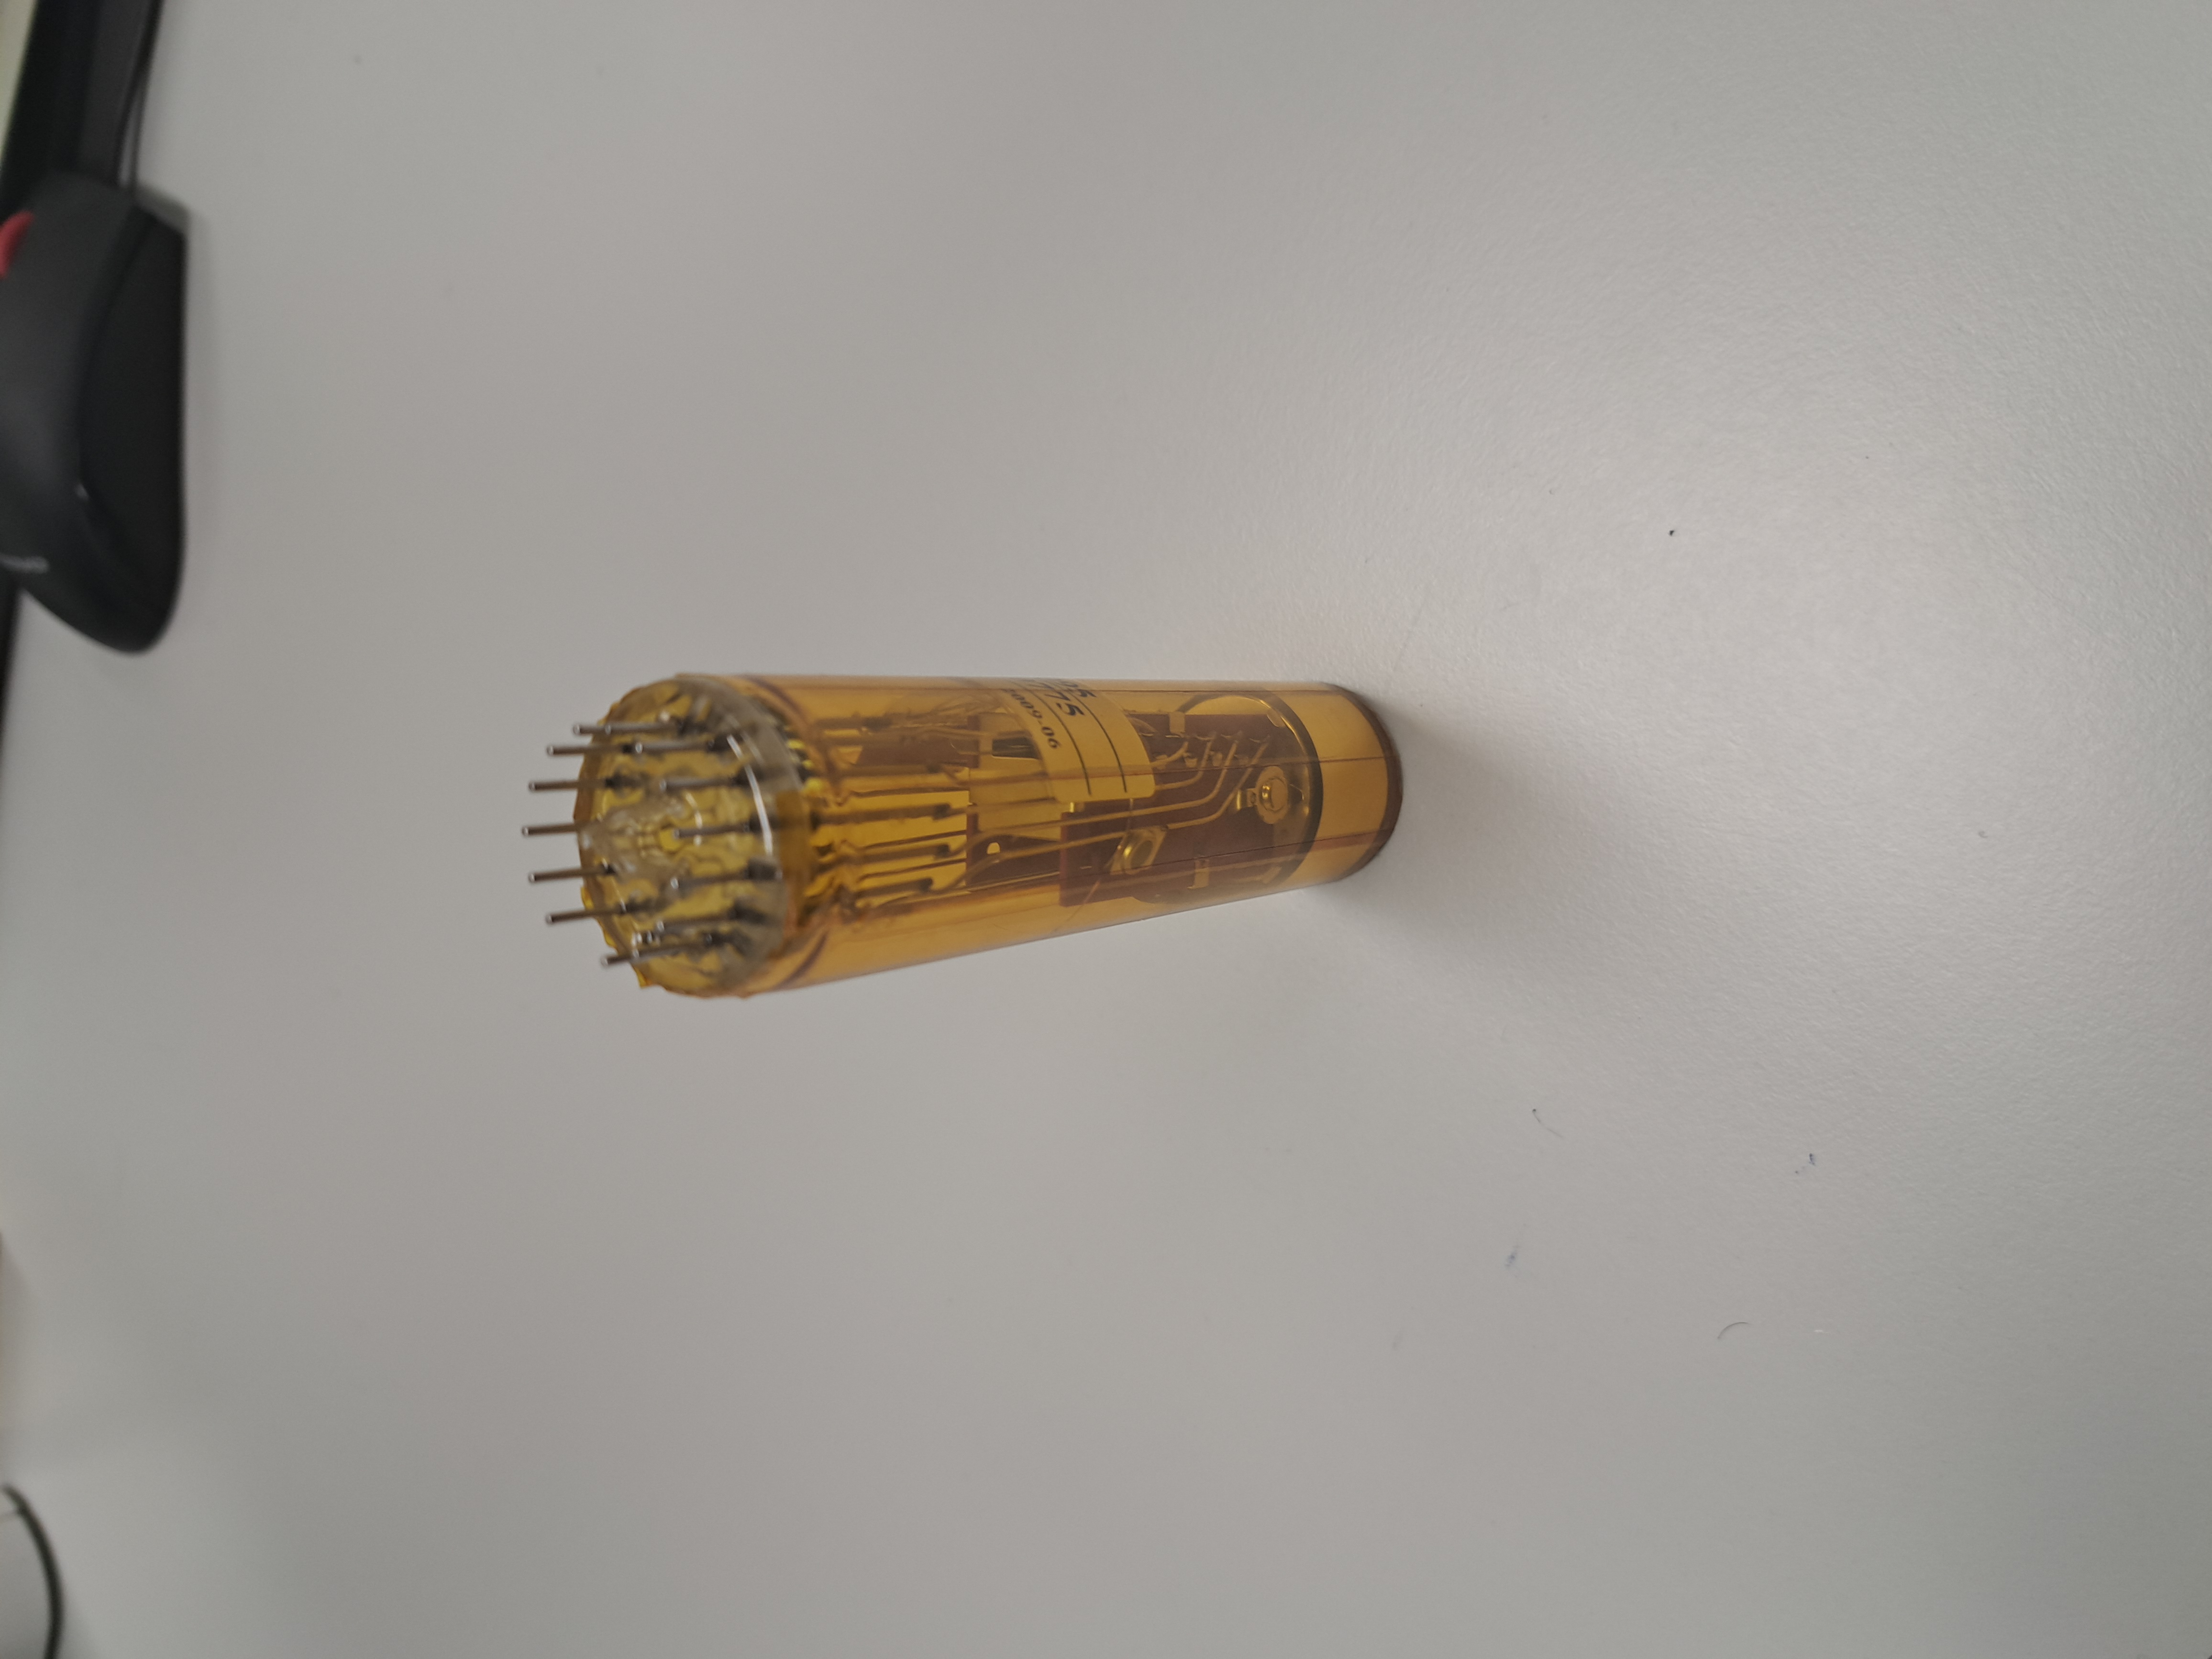
\includegraphics[width=0.7\textwidth]{img/photo/PMT.jpg}
        \caption[Photo d'un tube photomultiplicateur]{Photo d'un tube photomultiplicateur. Noter la fêlure à gauche de l'étiquette. Dimension~: diamètre 29*114~mm}
        \label{fig_PMT}
    \end{subfigure}
\end{figure}
\begin{description}
    \item[Un crystal NaI] Ce cristal a la propriété d'absorber les photons haut énergie des rayons gamma pour les réémettre comme des photons plus basse énergie (voir partie gauche de la \cref{fig_detecteur_gamma} et \cref{fig_Nai})~\cite{site:explication_NaI}
    \item[Un tube photomultiplicateur]ce tube permet de convertir un photon en un photoélectron qui est ensuite multiplié par le tube pour être converti en signaux électriques. (Voir partie droite de la \cref{fig_detecteur_gamma} et \cref{fig_PMT})~\cite{site:explication_NaI}
\end{description}
À la demande du client (Somaïr), une sonde basse a été incluse dans le projet pour permettre de faire des mesures aux niveaux du sol comme elle était faite avant (voir\ref{}). %photo et section
Les études internes montrent que les mesures les plus fiables sont faites à partir de la sonde haute donc la décision a été prise d'inclure les deux. À l'heure actuel, selon les données enregistrées par la sonde, 68,5~\% des mesures sont faits à partir de la sonde haute et 29~\% à partir de la sonde basse. Les autres mesures sont faites avec une combinaison des deux.

\subsection{Le GPS différentiel}
\label{ssec_Gps_differenciel}
Pour que la CanOp puisse fonctionner correctement, il faut qu'elle soit située très précisément ($\pm$ 10~cm sur les axes x et y et $\pm$ 1~cm sur les axes z), or un GPS classique n'arrive qu’a atteindre $\pm$~3~m horizontalement et $\pm$ 5~m verticalement dus notamment aux perturbations atmosphériques que subisse les signaux. 
\begin{figure}
    \centering
    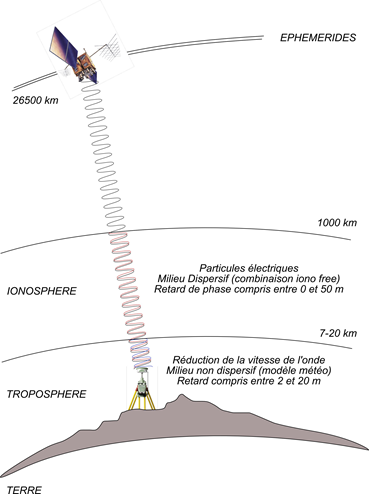
\includegraphics[height=0.5\textwidth]{img/she/GPS-mode-Naturel-5-10m.png}
    \caption[Source d'erreur des GPS]{Schéma présentant les sources d'erreur des GPS. Source~: Orphéon}
    \label{fig_GPS_error_source}
\end{figure}

Une des solutions possibles pour contourner ces problèmes est d'utiliser un GPS différentiel. Le principe de fonctionnement est simple, une station fixe à proximité de notre zone de mesure reçoit également les signaux GPS et en connaissant sa position précise peuvent calculer et transmettre les corrections nécessaires. \cite{site:GPS_diff}
\begin{figure}
    \centering
    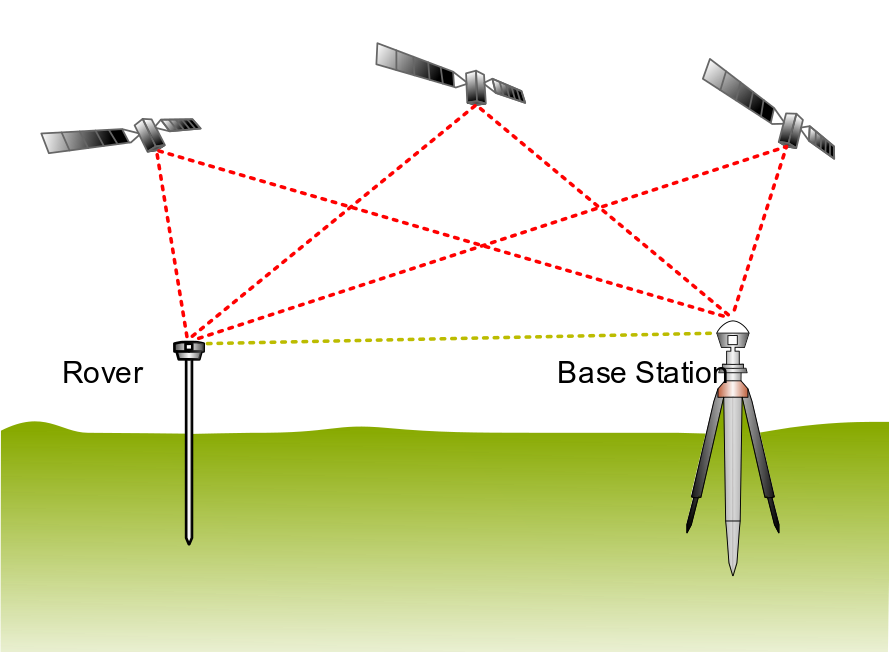
\includegraphics[width=0.5\textwidth]{img/she/Real_time_kinematic.png}
    \caption[Shema d'un systeme GPS differenciel]{Schéma d'un système GPS différentiel. Source~: \href{https://commons.wikimedia.org/wiki/File:Real_time_kinematic.svg}{TS Eriksson}, \href{https://creativecommons.org/licenses/by-sa/4.0}{CC BY-SA~4.0}, via Wikimedia Commons}
    \label{fig_RTK}
\end{figure}

\subsection{L'électronique}

    
\input{tex/Analyse_donnée}
\section{Amélioration de la CanOp}

Un des probleme majeur de la CanOp reste son poids relativement conséquent de 5,5~kg. Ce poids peut paraitre leger mais les operatuer doive porter les sonde a bout de bras pendant un shift de 8~hr sous le soleil avec une temperature qui monte regulierement au dessus de 40°C. Deja lors de sa conception on avez envisager de changer l'armature d'aluminum a de la fibre de carbon. 

Une grosse partie de mon travail a donc etait d'etudier et de proposer de solution a ce probleme. Assez rappidement trois avenue d'ameliration sont apparue.
\begin{enumerate}
    \item Alleger le gps 
    \item Alleger les sonde
    \item Repartir l'effort sur l'operateur
\end{enumerate}

\subsection{Allerger le Gps}
Actuellemnt le GPS est une piece monolitique fourit par Ophelia (voir \cref{ssec:Gps_differenciel}) qui calcule en interne la position corriger de la sonde. Une solution pourrait etre de fracturer le differnt partie du GPS et de delocaliser le calcule de la position et de sa correction a appliqué depuis la tablette de l'operateur en laissant l'antenne sur la sonde. D'autre solution a partir de puce integrer pourrait egalemetn mené a des econmie de poids.

\subsection{Alleger les sonde}
Les sonde sur les CanOp sont des sonde en deux piece composer d'un crystal scintilateur et d'un detectuer (ici un photomultiplier tube) (voir \cref{ssec:sonde}). C'est sonde sont relativement lourde et ne sont pas solidaire ce qui pose des problement de deconcetion accidentel et d'infiltration de poussiere/d'eau. 
J'ai donc chercher des sonde qui pourrait atre plus etanche et ou plus leger. En fesant c'est rechecher je suis tomber par accident sur des capteur solide state SiPM qui pourrait remplacer les tube photomultiplicateur. Ces composant sont devenue un remplacement viable de PMT que très recament et n'était donc pas diposible pour la V1 de la CanOp. C'est compossant present de nombreaux avantage:
\begin{itemize}
    \item plus leger
    \item peu cher a fabriquer en mass (capitalization sur les avancer faite en lithographie)
    \item moins cher
    \item Basse tenssion (5~V vs 1000-2000~V pour les PMT) $\rightarrow$ simplification des electronique
\end{itemize}

Ces avantage permet de produire des sonde gamma pesant 25~g\cite{} pour les plus petit comparer a environ 150~g\cite{} pour les sonde classic. Deplus ces sonde sont bien plus facile a rendre ettenche car il n'y a plus besoin de separer l'ecltronique du crystal.

\section{Les SiPM, un détecteur de lumière}
Au plus simple, un SiPM est un composant électronique qui permet de détecter de la lumière.

Un SiPM est une puce de silicium qui contrairement au processeur qui sont composés de transistors, est composé d'une multitude de photodiodes. Une photodiode est un composant électronique qui permet de convertir de la lumière en courant électrique. C'est notamment ce qui est à utiliser dans les cellules photovoltaïques des panneaux solaires. Ici, les photodiodes vont plutôt être optimisées pour détecter des photons que pour générer de l'électricité. 

En temps normal, une jonction p-n est un assemblage de deux matériaux semi-conducteurs qui agisse comme une diode (voir \cref{fig_pn_diode}). En choisissant judicieusement ses matériaux et en lui appliquant une tension dans son sens conventionnelle, on peut obtenir l'émission de lumière. C'est le principe de la LED. En revanche, si l’on applique une tension dans le sens inverse alors le courant ne peut plus circuler, car c'est une diode. Quand un photon d'une énergie suffisante vient frapper la jonction, il va libérer un électron qui va créer un courant électrique proportionnel au nombre de photons qui entre. C'est le principe de la photodiode.

Notre détecteur peut être plus sensible si nous augmentons la tension alors nous commençons à observer un phénomène d'avalanche. En effet, quand une paire électron-trou est créée, elle va accélérer dans le champ électrique et libéré d'autre paire électron-trou. C'est le principe du photodétecteur avalanche (APD)
(avalanche photodetector), mais nous arrivons rapidement a une limite~; à une certaine tension, dite la tension de claquage, la diode va se mettre a conduire dans le sens inverse. Dans ce cas, le photon que nous détecterons en premier créera un courant qui s'entretiendra tout seul. Pour empêcher cela, il faut donc limiter le courant du signal. Dans le cas des SiPM, cela est fait avec une résistance et une accumulatrice pour former ce qu'on appellera un SPAD (Single photon avalanche diode).

Dans un SiPM, nous allons relier en parallèle des centaines, voir des milliers de ces SPAD (voir \cref{fig_SiPM}). Ainsi, on augmente la surface de détection pour un photon. Actuellement, dans le commerce, la taille la plus grande de SiPM disponible est de 8~mm*8~mm\cite{}. En couplant plusieurs SiPM en parallèle, on peut donc détecter des photons sur une surface plus grande.

\begin{figure}
    \centering
    % \begin{subfigure}{0.45\textwidth}
    %     \centering
    %     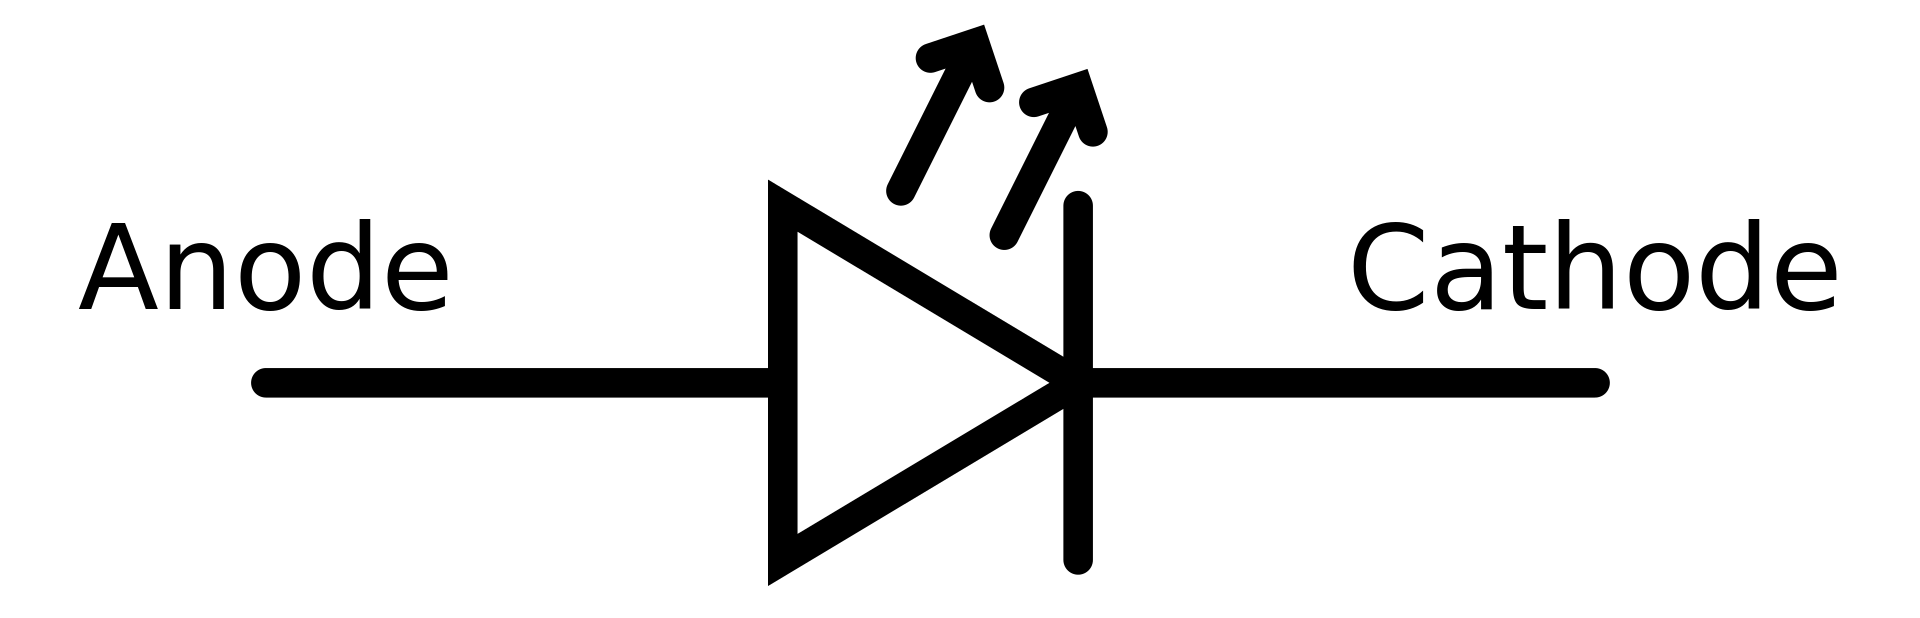
\includegraphics[width=\textwidth]{img/she/LED_symbol.svg.png}
    %     \captionsetup{width=.85\textwidth}
    %     \caption{Source: \href{https://commons.wikimedia.org/wiki/File:LED_symbol.svg}{Omegatron}, \href{https://creativecommons.org/licenses/by-sa/3.0}{CC BY-SA 3.0}, via Wikimedia Commons}
    %     \label{fig_LED_elec_symbol}
    % \end{subfigure}
    % \begin{subfigure}{0.45\textwidth}
    %     \centering
    %     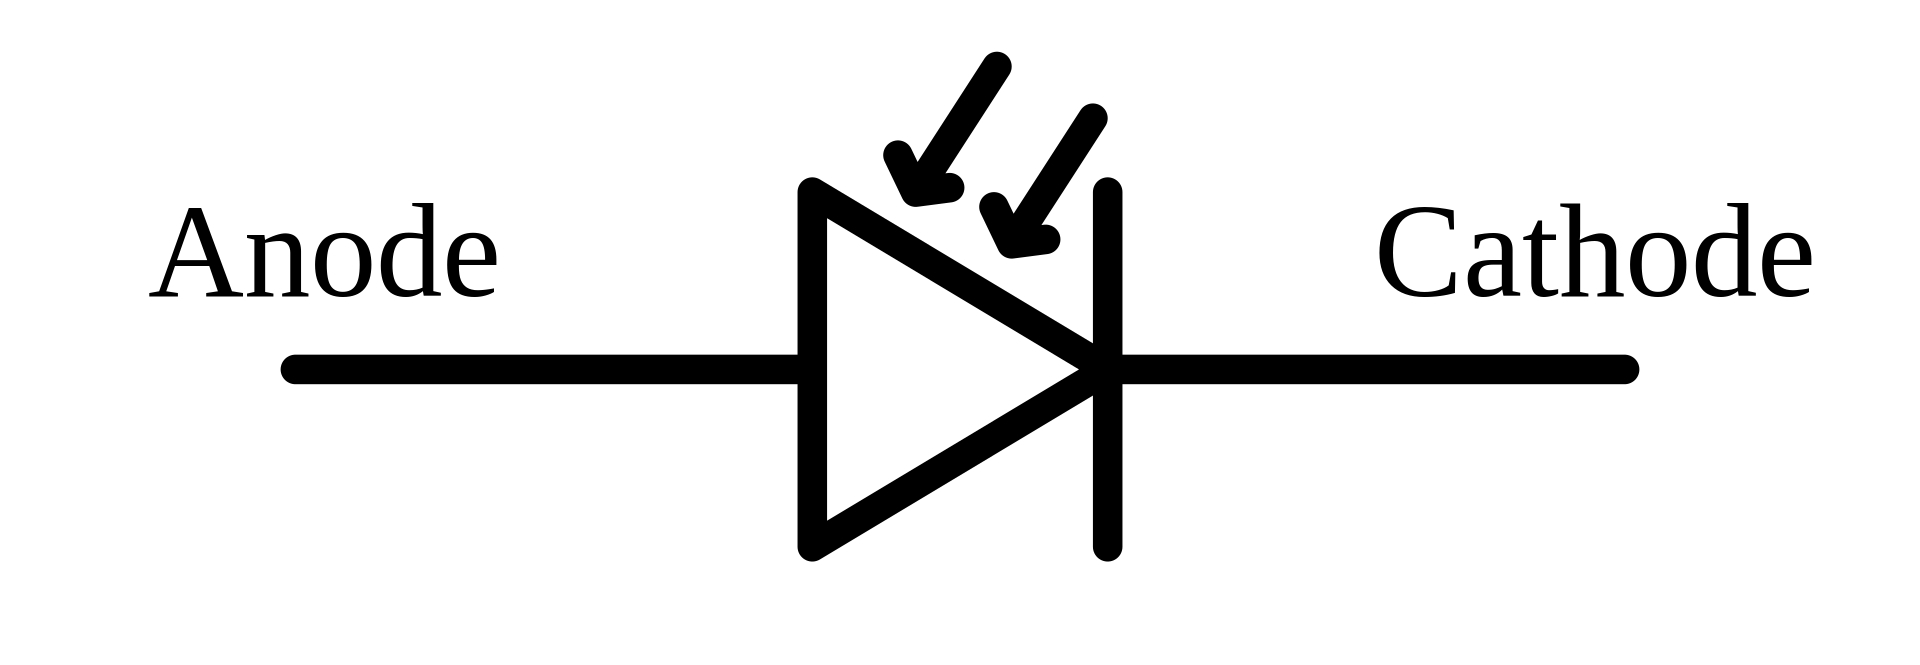
\includegraphics[width=0.85\textwidth]{img/she/Photodiode_symbol.svg.png}
    %     \captionsetup{width=.85\textwidth}
    %     \caption{Source: \href{https://commons.wikimedia.org/wiki/File:Photodiode_symbol.svg}{Simone Biancolilla}, \href{https://creativecommons.org/licenses/by-sa/3.0}{CC BY-SA 3.0}, via Wikimedia Commons}
    %     \label{fig_photodiode_elec_symbol}
    % \end{subfigure}
    \begin{subfigure}[c]{0.45\textwidth}
        \centering
        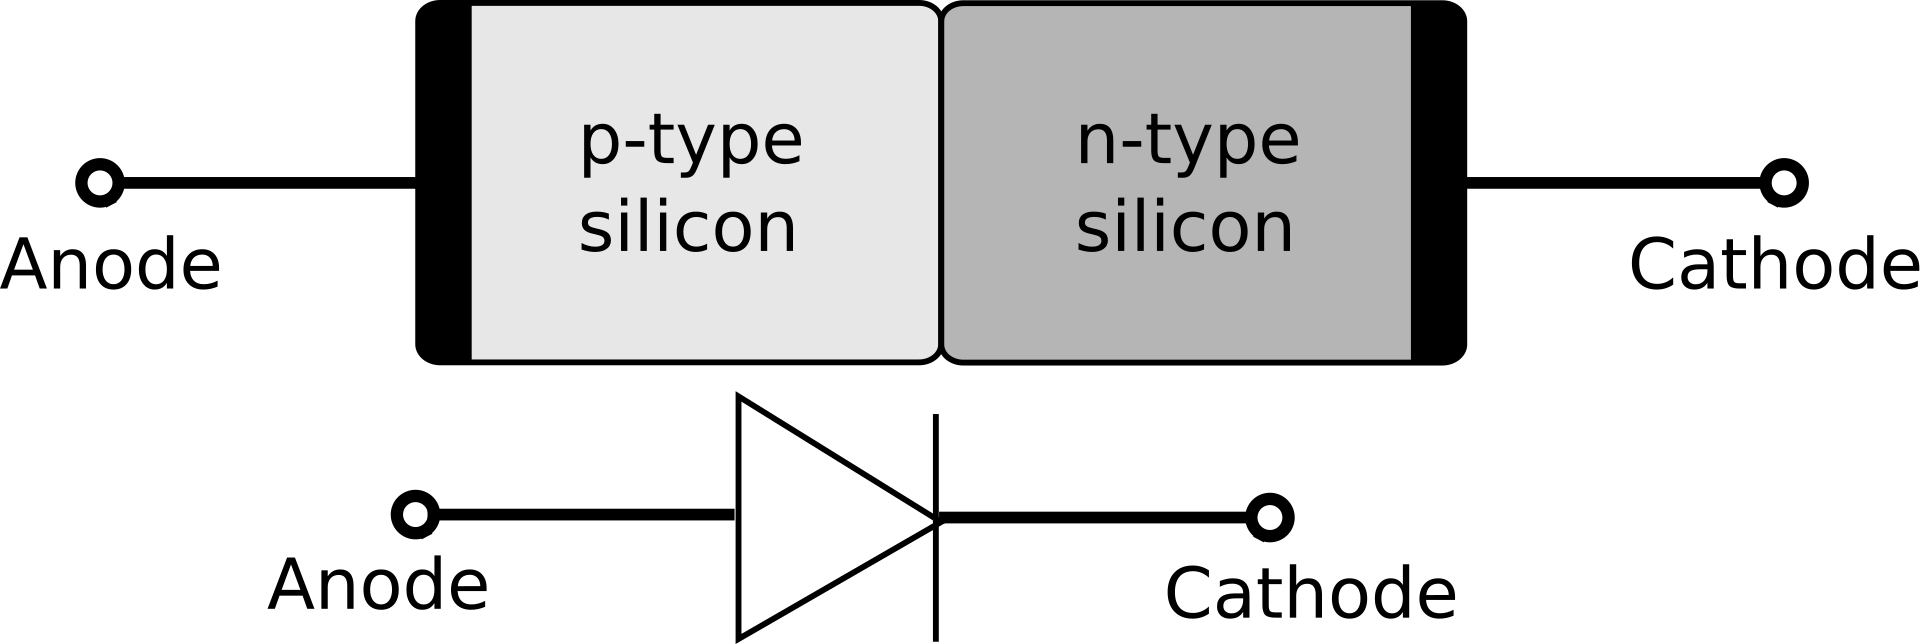
\includegraphics[trim= 0 -585 0 -585, width=0.85\textwidth]{img/she/1920px-PN_diode_with_electrical_symbol.svg.png}
        \captionsetup{width=.85\textwidth}
        \caption{Schéma montrant l'équivalence entre une jonction P-N et une diode. Source~: \href{https://commons.wikimedia.org/wiki/File:PN_diode_with_electrical_symbol.svg}{Raffamaiden}, \href{https://creativecommons.org/licenses/by-sa/3.0}{CC BY-SA~3.0}, via Wikimedia Commons}
        \label{fig_pn_diode}
    \end{subfigure}
    \begin{subfigure}[c]{0.45\textwidth}
        \centering
        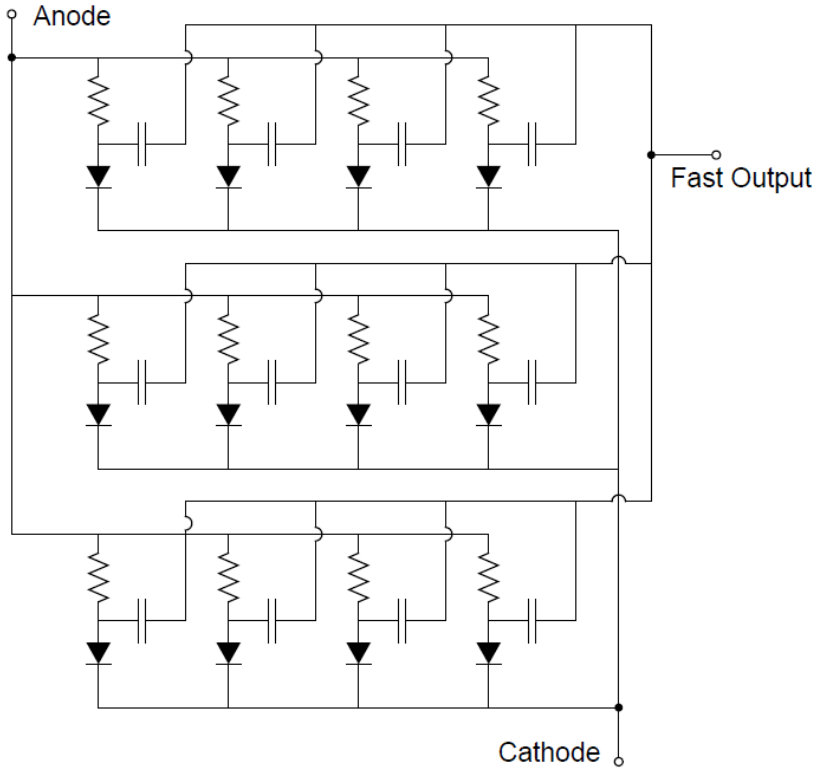
\includegraphics[width=0.85\textwidth]{img/she/SiPM_arithecture.png}
        \captionsetup{width=.85\textwidth}
        \caption{Schéma d'un SiPM. Les diodes sont des diodes photoavalanche. On ne représente pas tous les modules. Source~: \href{https://websites.umich.edu/~ners580/ners-bioe_481/lectures/pdfs/2017-02-.pdf}{An Intro to SiPM, SensL}}
        \label{fig_SiPM}
    \end{subfigure}
    \caption[Composition d'un SiPM]{Composition d'un SiPM}
\end{figure}

\section{Simulation}
Une difference etre les tube photomultiplicateur et les SiPM est que les tube photomultiplicateur ont une zone de detection en forme de rond alors que les SiPM ne peuve que etre produit en carré et donc les une zone de detection carré. Cela implique donc un changement de forme de cristal. Pour s'assurer que les ancien cristaux et les nouveaux se comporte de la meme maniere, nous allons faire une simulation. Les cristaux NaI utiliser actuelment sont des cylindre de 28mm de diametre et 50mm de hauteur. Pour que les nouveaux critaux cuboide rentre dans le boitier, ils doive avoir une longeur et une largeur de 20mm et pour que le volume, et donc normalement le nombre de detection, reste le meme, ils doive avoir une hauteur de 76.96mm. Nous testeron egalement un cristal avec un hauteur de 75mm pour voir si la petit difference de volume a un impact sur les resultats.
\pgfplotstableread[row sep=\\,col sep=&]{
    cristal                                                  & Serie 1 & Serie 2 & error_1   & error_2\\
    Cristal cylindrique                                      & 1430.18 & 955.978 & 563.49092 & 372.5446266 \\
    Cristal cuboide (\qtyproduct{20x20x76.96}{\milli\metre}) & 2221.99 & 963.492 & 709.925805 & 255.1326816 \\
    Cristal cuboide (\qtyproduct{20x20x75}{\milli\metre})    & 2092.62 & 1502.45 & 400036.744991191 & 95048.3096001287 \\
}\datatable
\begin{figure}
    \centering
    % 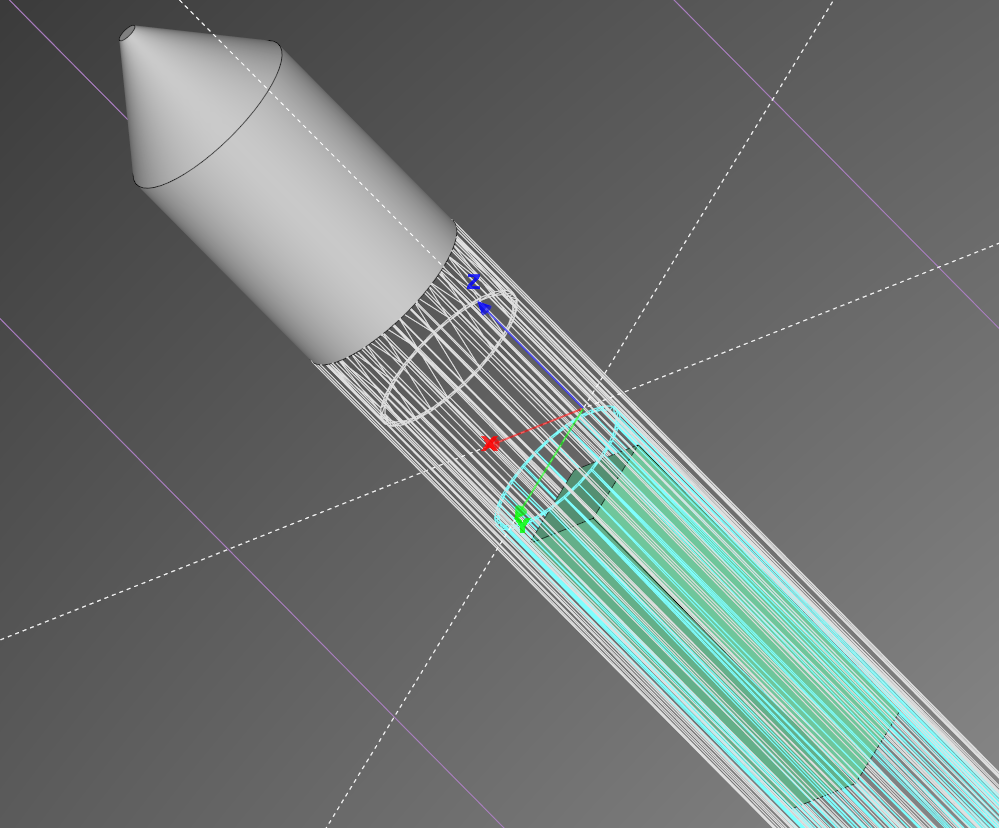
\includegraphics[width=0.5\textwidth]{photo/sonde_carre_simu.PNG}
    \begin{subfigure}[t]{0.49\textwidth}
        \centering
        \begin{tikzpicture}[baseline=(current bounding box.north)] %allows to align the top of tikzpicture to the other subfigure
            \begin{axis}[
                    ybar,
                    enlarge y limits={value=0.15, upper},
                    width=1\textwidth,
                    legend style={at={(0.99,0.99)},
                            anchor=north east,legend columns=-1},
                    ylabel={Comptage (\unit{cps})},
                    ymin=0,
                    % ylabel shift = 0.1 \linewidth,
                    symbolic x coords={Cristal cylindrique,Cristal cuboide (\qtyproduct{20x20x76.96}{\milli\metre}),Cristal cuboide (\qtyproduct{20x20x75}{\milli\metre})},
                    xtick=data,
                    xticklabel style={text width=0.33\linewidth,anchor=north},
                ]
                \addplot table[x=cristal,y=Serie 1] {\datatable};
                \addplot table[x=cristal,y=Serie 2] {\datatable};
                \legend{Serie 1,Serie 2}
            \end{axis}
        \end{tikzpicture}    
        \caption{Comparaison des comptages entre les cristaux cylindrique et cuboide}
    \end{subfigure}
    \begin{subfigure}[t]{0.49\textwidth}
        \centering
        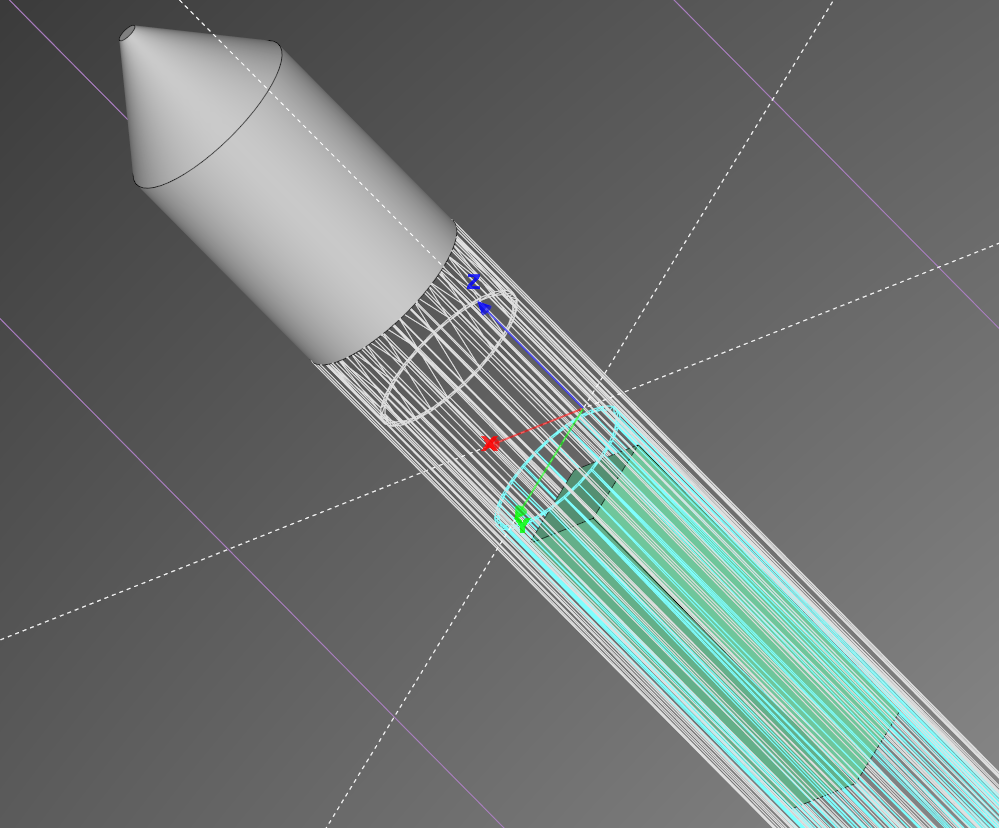
\includegraphics[width=0.9\textwidth]{photo/sonde_carre_simu.PNG}

        \caption{Capture d'ecran de la simulation d'un cristal cuboide}
        
    \end{subfigure}
\end{figure}

Un autre stagiare travailler sur des sujet de simulation et a donc pu faire ces simulation pour moi. Malheuresment il n'avait pas encore eu ses acces au serveur de calcul d'orano et donc a du les faire tourner a plus basse resolution sur sont ordinateur.


\section{Conclusion}

Ce stage m'a permis de découvrir le secteur de l'industrie minière et de l'uranium. J'ai observé comment les données sont utilisées pour optimiser la production et comment les nouvelles technologies sont évaluées pour améliorer les processus. J'ai également vu comment les différents services d'une entreprise collaborent pour atteindre un objectif commun. Ce stage m'a aussi permis de développer mes compétences en analyse de données et pour trouver des solutions technologiques.

J'ai le sentiment d'avoir beaucoup appris, tant sur le plan humain, que sur le plan technique. J'ai pu mobiliser et approfondir mes connaissances pour comprendre en détail le fonctionnement d'un SiPM. Dans la continuité de l'enseignement de l'Institut Villebon \textit{George Charpak} j'ai été amené à travailler en équipe et à résoudre de problème et ainsi, développer ces compétences. J'ai également découvert de nouveaux outils comme PowerBI et Pandas, qui me seront utiles dans le futur.
% \section{test}
% \label{test_label}
% hello world \cite{article:uranium-concentration} \cref{test_label}
% \bibliographystyle{nar}
% %\bibliographystyle{IEEEtran} % We choose the "plain" reference style
% \bibliography{refs} % Entries are in the refs.bib file
%https://prezi.com/view/FbRiFt9MbWPpmL9kAI9v/
\newpage
\AtNextBibliography{\small}
\printbibliography
\addcontentsline{toc}{section}{Bibliography}
\clearpage


\appendix
% \section{Bilan Personnel}


\section{Technique d'extraction}
Source: \href{https://www.cameco.com/businesses/mining-methods}{Cameco Mining Methods}

\subsection*{Boxhole Boring}
\label{ssec_boxbore}
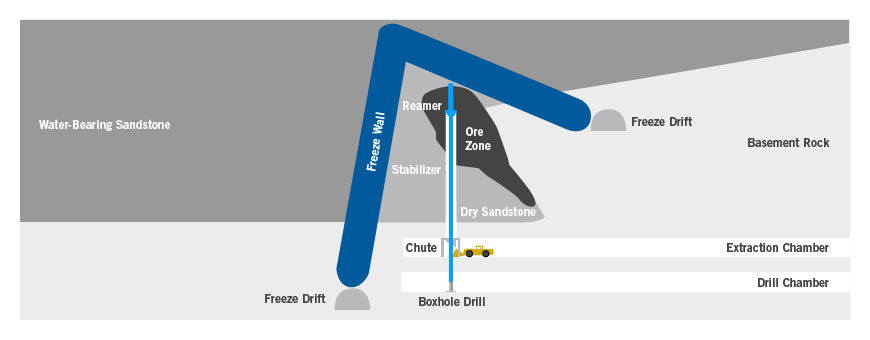
\includegraphics[width=0.9\textwidth]{img/cameco/3.0.1-1MiningMethods-Boxhole.jpg}

Boxhole boring is similar to the \nameref{ssec_raisebore}, but the drilling machine is located below the mineralization, so development is not required above the mineralization. From a drill chamber in waste rock below the ore, we drill a series of overlapping holes up through the ore zone and collect the falling ore from a chute in the extraction chamber. This method is currently being used at a few mines around the world, but had not been used for uranium mining prior to testing at McArthur River.
\subsection*{Blasthole Stoping}


Blasthole stoping involves establishing drill access above the mineralization and extraction access below the mineralization. The area between the upper and lower access levels (the stope) is then drilled off and blasted. The broken rock is collected on the lower level by line-of-sight remote-controlled scoop trams and transported to a grinding circuit. Once a stope is mined out, it is backfilled with concrete to maintain ground stability and allow the next stope in sequence to be mined. This mining method has been used extensively in the mining industry.
\subsection*{Jet Boring}
\label{ssec_jetbore}
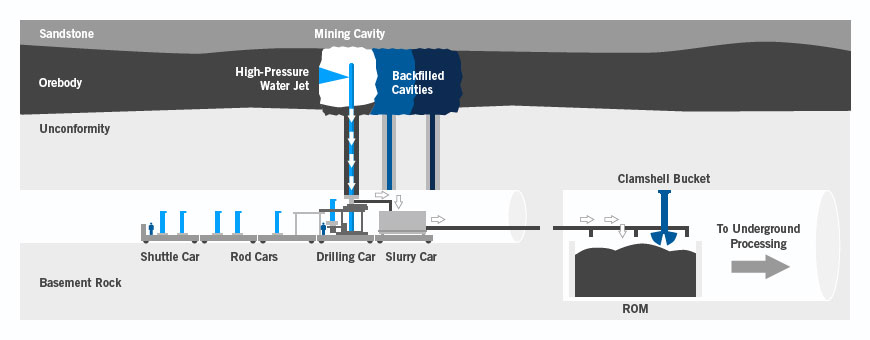
\includegraphics[width=0.9\textwidth]{img/cameco/3.0.1-2MiningMethods-JetBore.jpg}

Jet boring involves freezing the ore and surrounding rock in order to mine safely at Cigar Lake. Brine, chilled to -40C, is piped underground to the deposit. The brine is circulated through large pipes, freezing the surrounding rock in about one year. When ready, a mining machine bores through the frozen rock to create the production tunnel. The jet boring system enters this tunnel and drills a pilot hole through the orebody. Then the jet boring nozzle is inserted in the pilot hole and the system begins boring through the rock using a high-pressure jet of water. Loose ore is flushed down the pilot hole. After a series of processes, ore is pumped to the surface in a slurry form.

\href{https://www.cameco.com/businesses/mining-methods/jet-boring-video}{Watch video}
\subsection*{In Situ recovery}
\label{ssec_insitu}
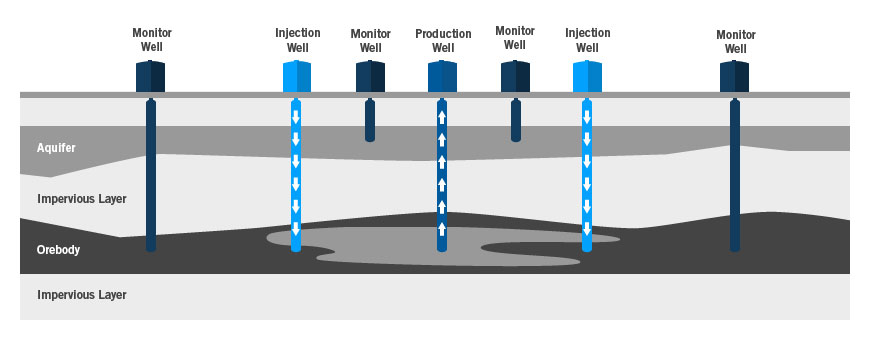
\includegraphics[width=0.9\textwidth]{img/cameco/3.0.1-3MiningMethods-ISR.jpg}

In situ recovery (ISR) methods are applied at our operations in the US and Kazakhstan to extract uranium contained in sandstone aquifers. In situ techniques involve circulation of solutions through ore-bearing formations to dissolve uranium and pump it to the surface for recovery. This approach results in minimal surface disturbance and produces no waste rock or mill tailings.

\href{https://www.cameco.com/businesses/mining-methods/in-situ-recovery-video}{Watch video}
\subsection*{Raisebore Mining}
\label{ssec_raisebore}
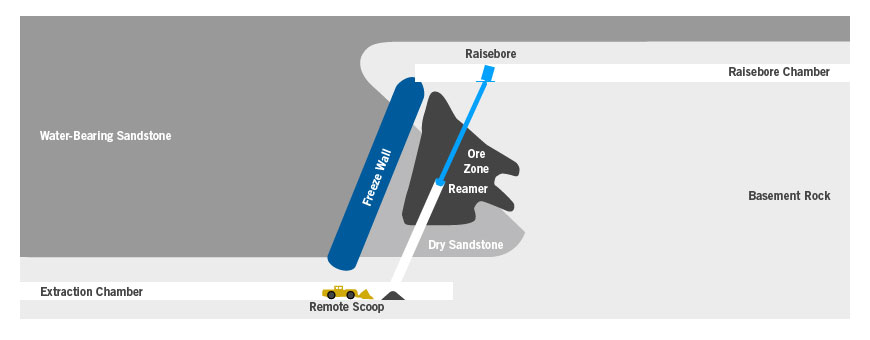
\includegraphics[width=0.9\textwidth]{img/cameco/3.0.1-4MiningMethods-Raisebore.jpg}

Raisebore mining is an innovative non-entry approach that we adapted to meet the unique challenges at McArthur River. From a raisebore chamber in waste rock above the ore, we drill a series of overlapping holes through the ore zone and collect the ore using remote-controlled scoop trams at the bottom of the raises. Once each raisebore hole is complete, we fill it with concrete. We have successfully used the raisebore mining method to extract more than 250 million lbs since we began mining in 1999.



\end{document}


